\documentclass[tikz,border=7pt]{standalone}
\usepackage{iftex}
\ifPDFTeX
  \PackageError{matrix-figure}{This figure requires XeTeX or Tectonic}{Compile with xelatex or tectonic.}
\fi
\usepackage{fontspec}
\usepackage{xeCJK}
\usepackage{amsmath}
\usepackage{unicode-math}
\usepackage{xcolor}
\usepackage{tikz}
\usetikzlibrary{arrows.meta,positioning}

\providecommand{\FigureUseLocalFonts}{0}
\ifnum\FigureUseLocalFonts=1
  \setmainfont{NotoSansCJKtc-Regular.otf}[Path=\FigureSansFontPath]
  \setsansfont{NotoSansCJKtc-Regular.otf}[Path=\FigureSansFontPath,BoldFont=NotoSansCJKtc-Bold.otf]
  \setCJKmainfont{NotoSansCJKtc-Regular.otf}[Path=\FigureSansFontPath]
  \setCJKsansfont{NotoSansCJKtc-Regular.otf}[Path=\FigureSansFontPath,BoldFont=NotoSansCJKtc-Bold.otf]
  \setmathfont{STIXTwoMath.otf}[Path=\FigureMathFontPath]
\else
  \setmainfont{Noto Sans CJK TC}
  \setsansfont{Noto Sans CJK TC}
  \setCJKmainfont{Noto Sans CJK TC}
  \setCJKsansfont{Noto Sans CJK TC}
  \setmathfont{STIX Two Math}
\fi

\definecolor{FigureInk}{HTML}{253142}
\definecolor{PanelFill}{gray}{0.96}
\definecolor{RowShade}{gray}{0.86}
\definecolor{ColumnShade}{gray}{0.74}
\definecolor{ResultShade}{gray}{0.58}
\definecolor{FocusShade}{gray}{0.68}
\definecolor{GuideShade}{gray}{0.80}

\newcommand{\MatrixCell}[2]{%
  \tikz[baseline=(value.base)]{\node[fill=#1,rounded corners=0.4pt,inner sep=2.2pt,
    minimum width=1.35em,minimum height=1.35em] (value) {$#2$};}%
}
\newcommand{\RowCell}[1]{\MatrixCell{RowShade}{#1}}
\newcommand{\ColumnCell}[1]{\MatrixCell{ColumnShade}{#1}}
\newcommand{\ResultCell}[1]{\MatrixCell{ResultShade}{#1}}
\newcommand{\FocusCell}[1]{\MatrixCell{FocusShade}{#1}}

\tikzset{
  figure/.style={font=\sffamily,text=FigureInk,>={Stealth[length=3.5mm,width=2.5mm]}},
  panel/.style={draw=FigureInk,line width=0.9pt,rounded corners=1.5mm,fill=PanelFill,align=center},
  flow/.style={-{Stealth},line width=1.05pt,draw=FigureInk},
}


\begin{document}
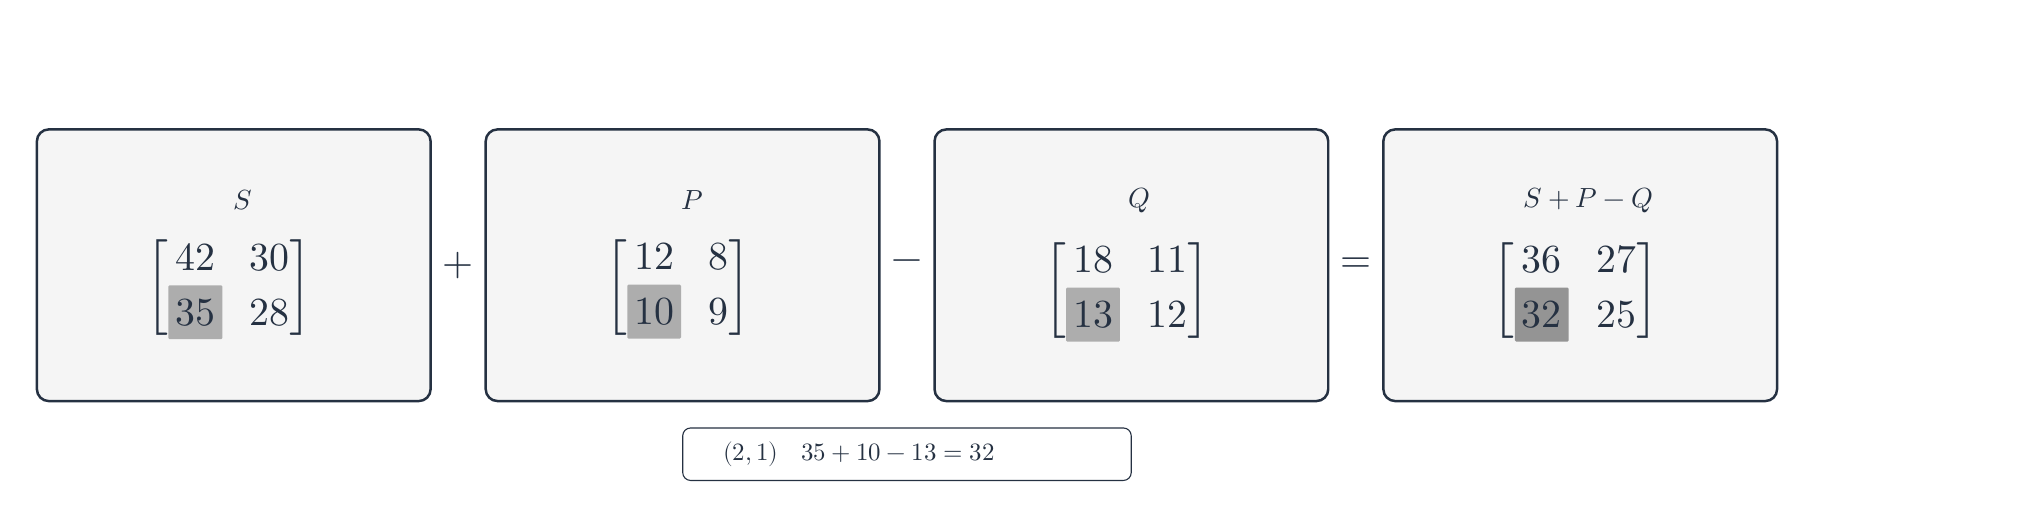
\begin{tikzpicture}[figure]
  \node[font=\bfseries\Large,align=center,text width=25cm] at (12.5,5.9)
    {同一索引的庫存逐項執行「期初＋進貨－銷售＝期末」};

  \node[panel,minimum width=5.0cm,minimum height=3.45cm] (S) at (2.5,3.0) {%
    \begin{minipage}{4.4cm}\centering
      \textbf{期初 $S$}\\[8pt]
      \Large$\begin{bmatrix}42&30\\\FocusCell{35}&28\end{bmatrix}$
    \end{minipage}
  };
  \node[font=\Large] at (5.35,3.0) {$+$};
  \node[panel,minimum width=5.0cm,minimum height=3.45cm] (P) at (8.2,3.0) {%
    \begin{minipage}{4.4cm}\centering
      \textbf{進貨 $P$}\\[8pt]
      \Large$\begin{bmatrix}12&8\\\FocusCell{10}&9\end{bmatrix}$
    \end{minipage}
  };
  \node[font=\Large] at (11.05,3.0) {$-$};
  \node[panel,minimum width=5.0cm,minimum height=3.45cm] (Q) at (13.9,3.0) {%
    \begin{minipage}{4.4cm}\centering
      \textbf{銷售 $Q$}\\[8pt]
      \Large$\begin{bmatrix}18&11\\\FocusCell{13}&12\end{bmatrix}$
    \end{minipage}
  };
  \node[font=\Large] at (16.75,3.0) {$=$};
  \node[panel,minimum width=5.0cm,minimum height=3.45cm] (C) at (19.6,3.0) {%
    \begin{minipage}{4.4cm}\centering
      \textbf{期末 $S+P-Q$}\\[8pt]
      \Large$\begin{bmatrix}36&27\\\ResultCell{32}&25\end{bmatrix}$
    \end{minipage}
  };

  \node[draw=FigureInk,rounded corners=1mm,fill=white,inner xsep=9pt,inner ysep=5pt,
        font=\small] at (11.05,0.6)
    {第 $(2,1)$ 元：$35+10-13=32$；每個位置都使用同一條更新規則。};
\end{tikzpicture}
\end{document}
